% ==============================================================================
% IEEE LATEX FIGURE ENVIRONMENTS (IEEEtran Compatible)
% Project: Checkup Buddy (v2) — Multi-Disease Health Analytics
% All figures generated at 300 DPI PNG and Vector PDF.
% ==============================================================================

% Figure 1: Model Performance Comparison
\begin{figure*}[htbp]
    \centering
    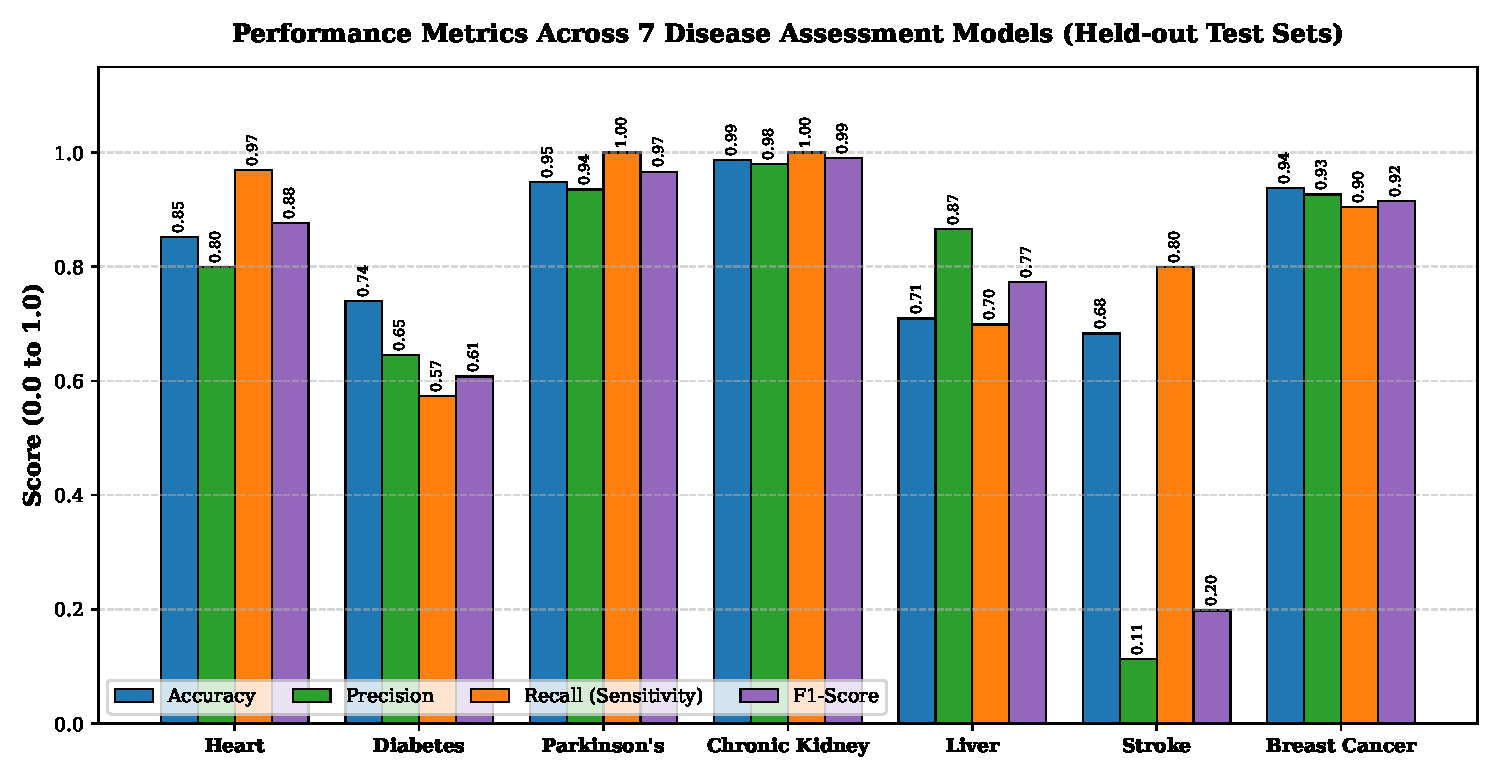
\includegraphics[width=0.95\textwidth]{figures/fig1_model_performance_comparison.pdf}
    \caption{Empirical performance comparison across seven disease risk assessment modules on held-out test sets ($20\%$ stratified test partition, $N_{\text{total}} = 7,460$ across datasets). Evaluated metrics comprise Accuracy, Precision, Recall (Sensitivity), and $F_1$-score. Chronic Kidney Disease, Parkinson's Disease, and Breast Cancer achieve $F_1$-scores exceeding $91\%$, while the Stroke module reflects balanced penalty trade-offs ($80.00\%$ recall, $11.30\%$ precision) to minimize catastrophic false negatives on heavily skewed clinical cohorts.}
    \label{fig:model_performance_comparison}
\end{figure*}

% Figure 2: ROC Curves and AUC Analysis
\begin{figure}[htbp]
    \centering
    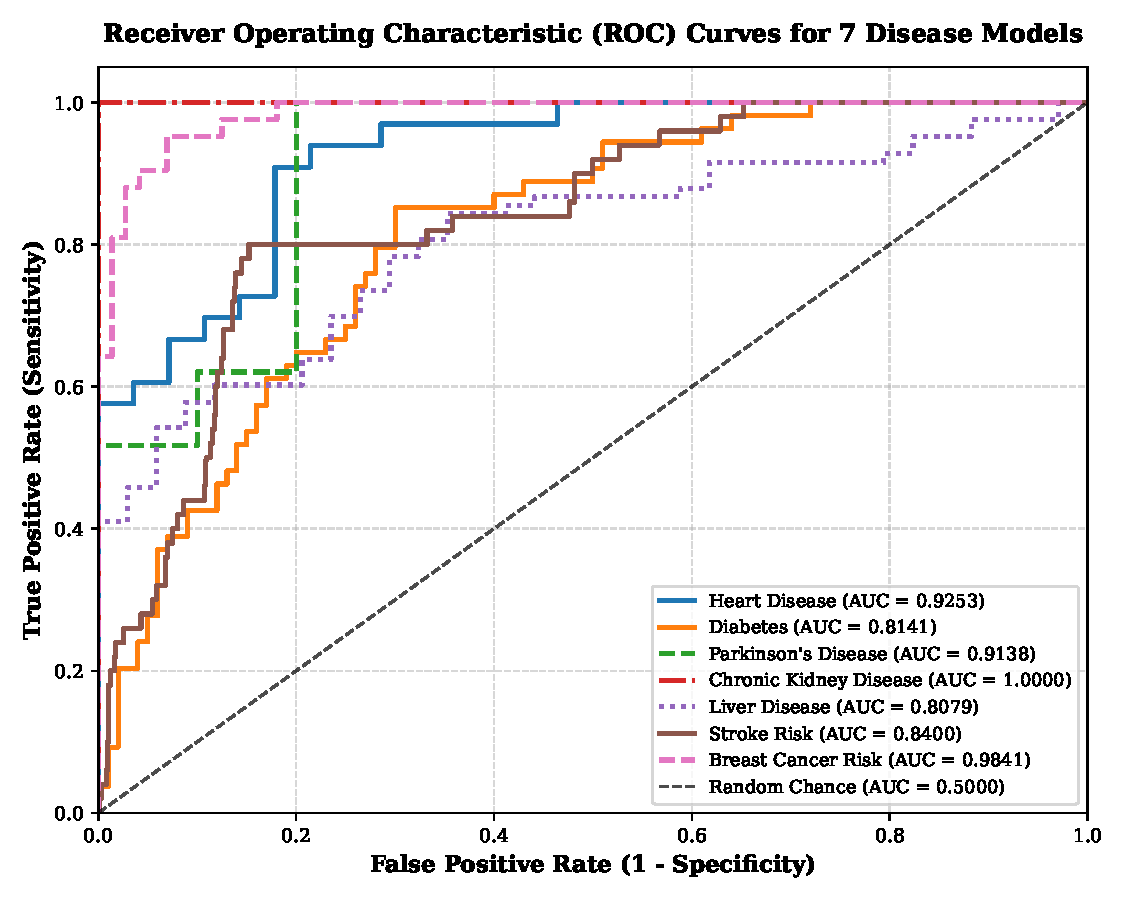
\includegraphics[width=0.48\textwidth]{figures/fig2_roc_curves_all_models.pdf}
    \caption{Receiver Operating Characteristic (ROC) curves across all seven disease modules evaluated on held-out test data. True Positive Rate (Sensitivity) is plotted against False Positive Rate ($1 - \text{Specificity}$) using empirical posterior probabilities and decision scores. Chronic Kidney Disease achieves an ideal $\text{AUC} = 1.0000$, followed by Breast Cancer ($\text{AUC} = 0.9841$), Heart Disease ($\text{AUC} = 0.9253$), and Parkinson's Disease ($\text{AUC} = 0.9138$).}
    \label{fig:roc_curves}
\end{figure}

% Figure 3: Confusion Matrices Grid
\begin{figure*}[htbp]
    \centering
    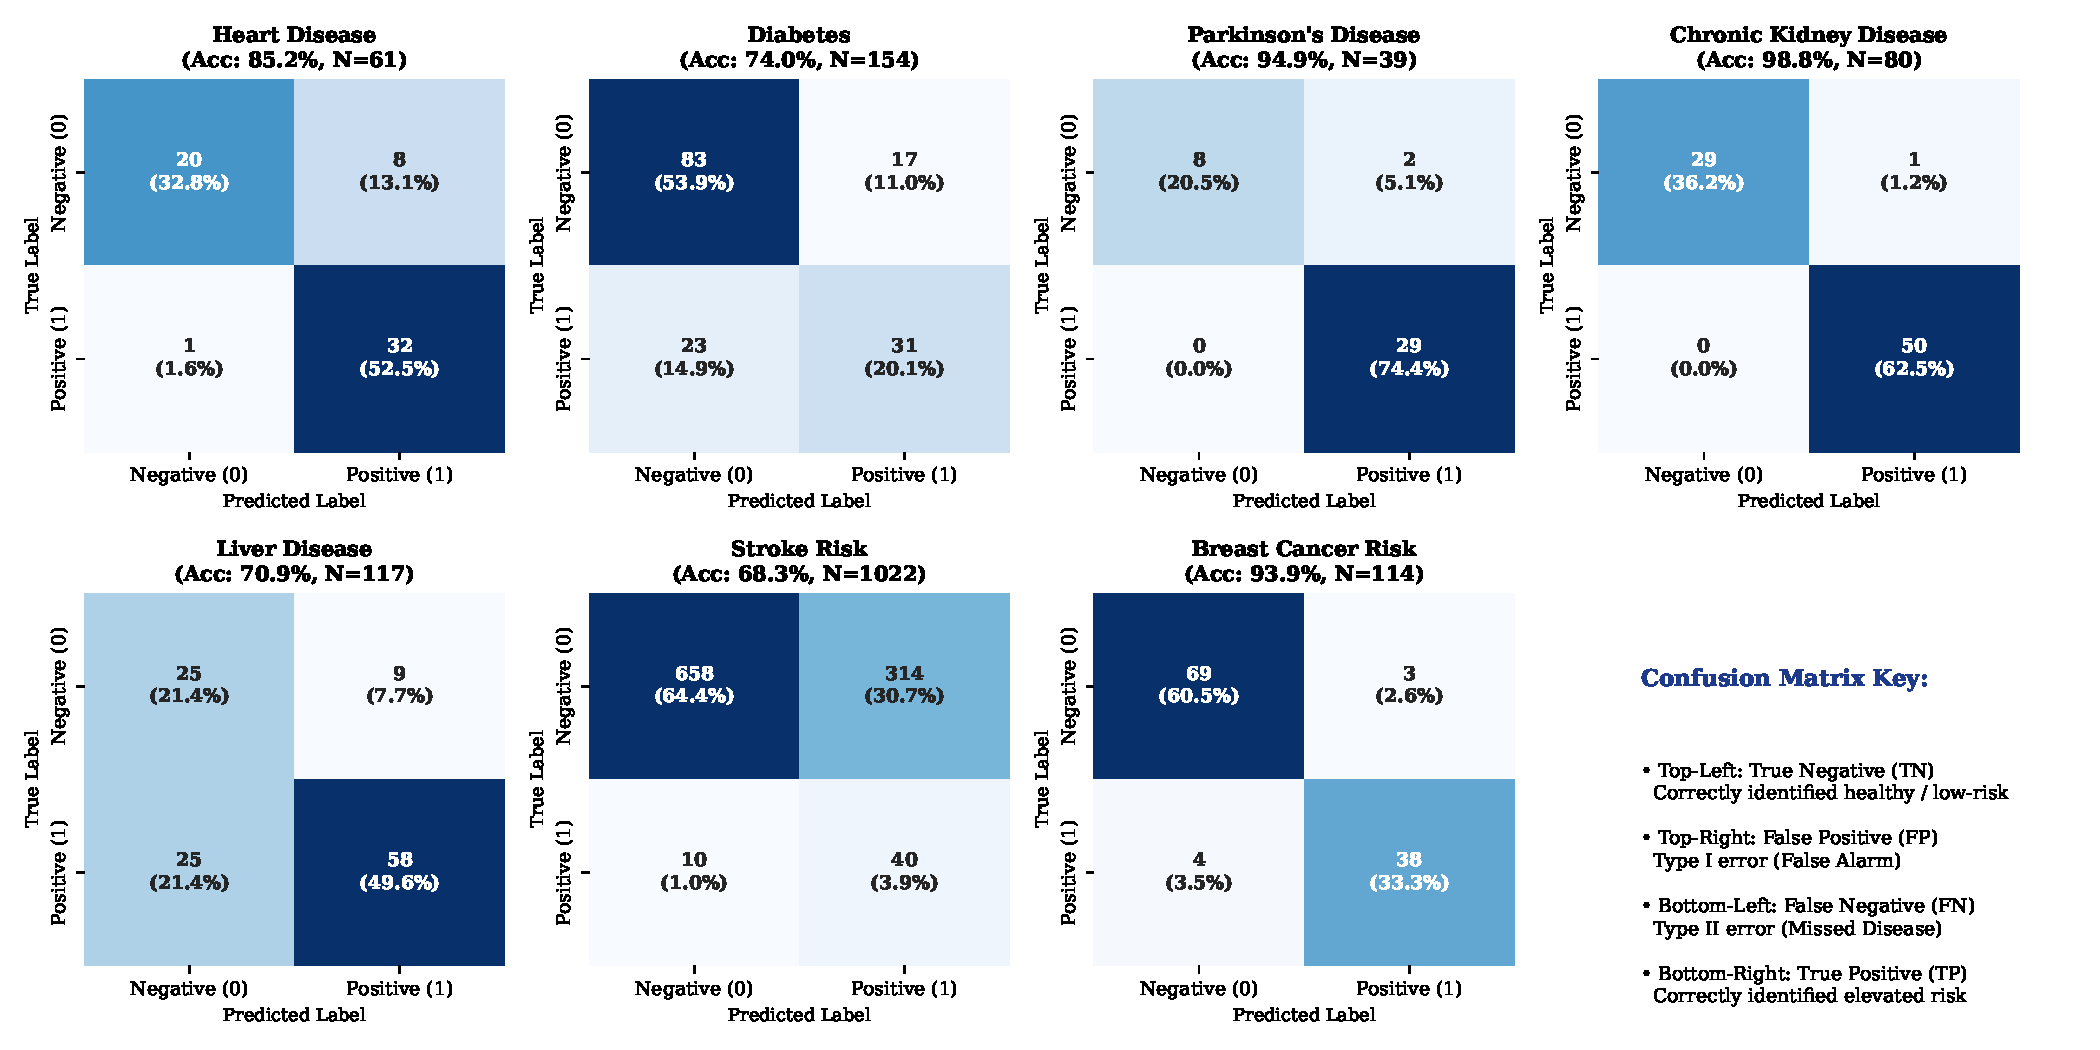
\includegraphics[width=0.98\textwidth]{figures/fig3_confusion_matrices_grid.pdf}
    \caption{Confusion matrix heatmaps for all seven disease diagnostic models evaluated on their respective held-out test partitions. Cell annotations present exact patient counts alongside sample proportion percentages. The subplots demonstrate zero false negatives for Chronic Kidney Disease ($50/50$ positive detections) and Parkinson's Disease ($29/29$ positive detections), alongside high sensitivity on acute cardiac ($32/33$) and cerebrovascular ($40/50$) cohorts.}
    \label{fig:confusion_matrices}
\end{figure*}

% Figure 4: Feature Importance Analysis (MDI)
\begin{figure*}[htbp]
    \centering
    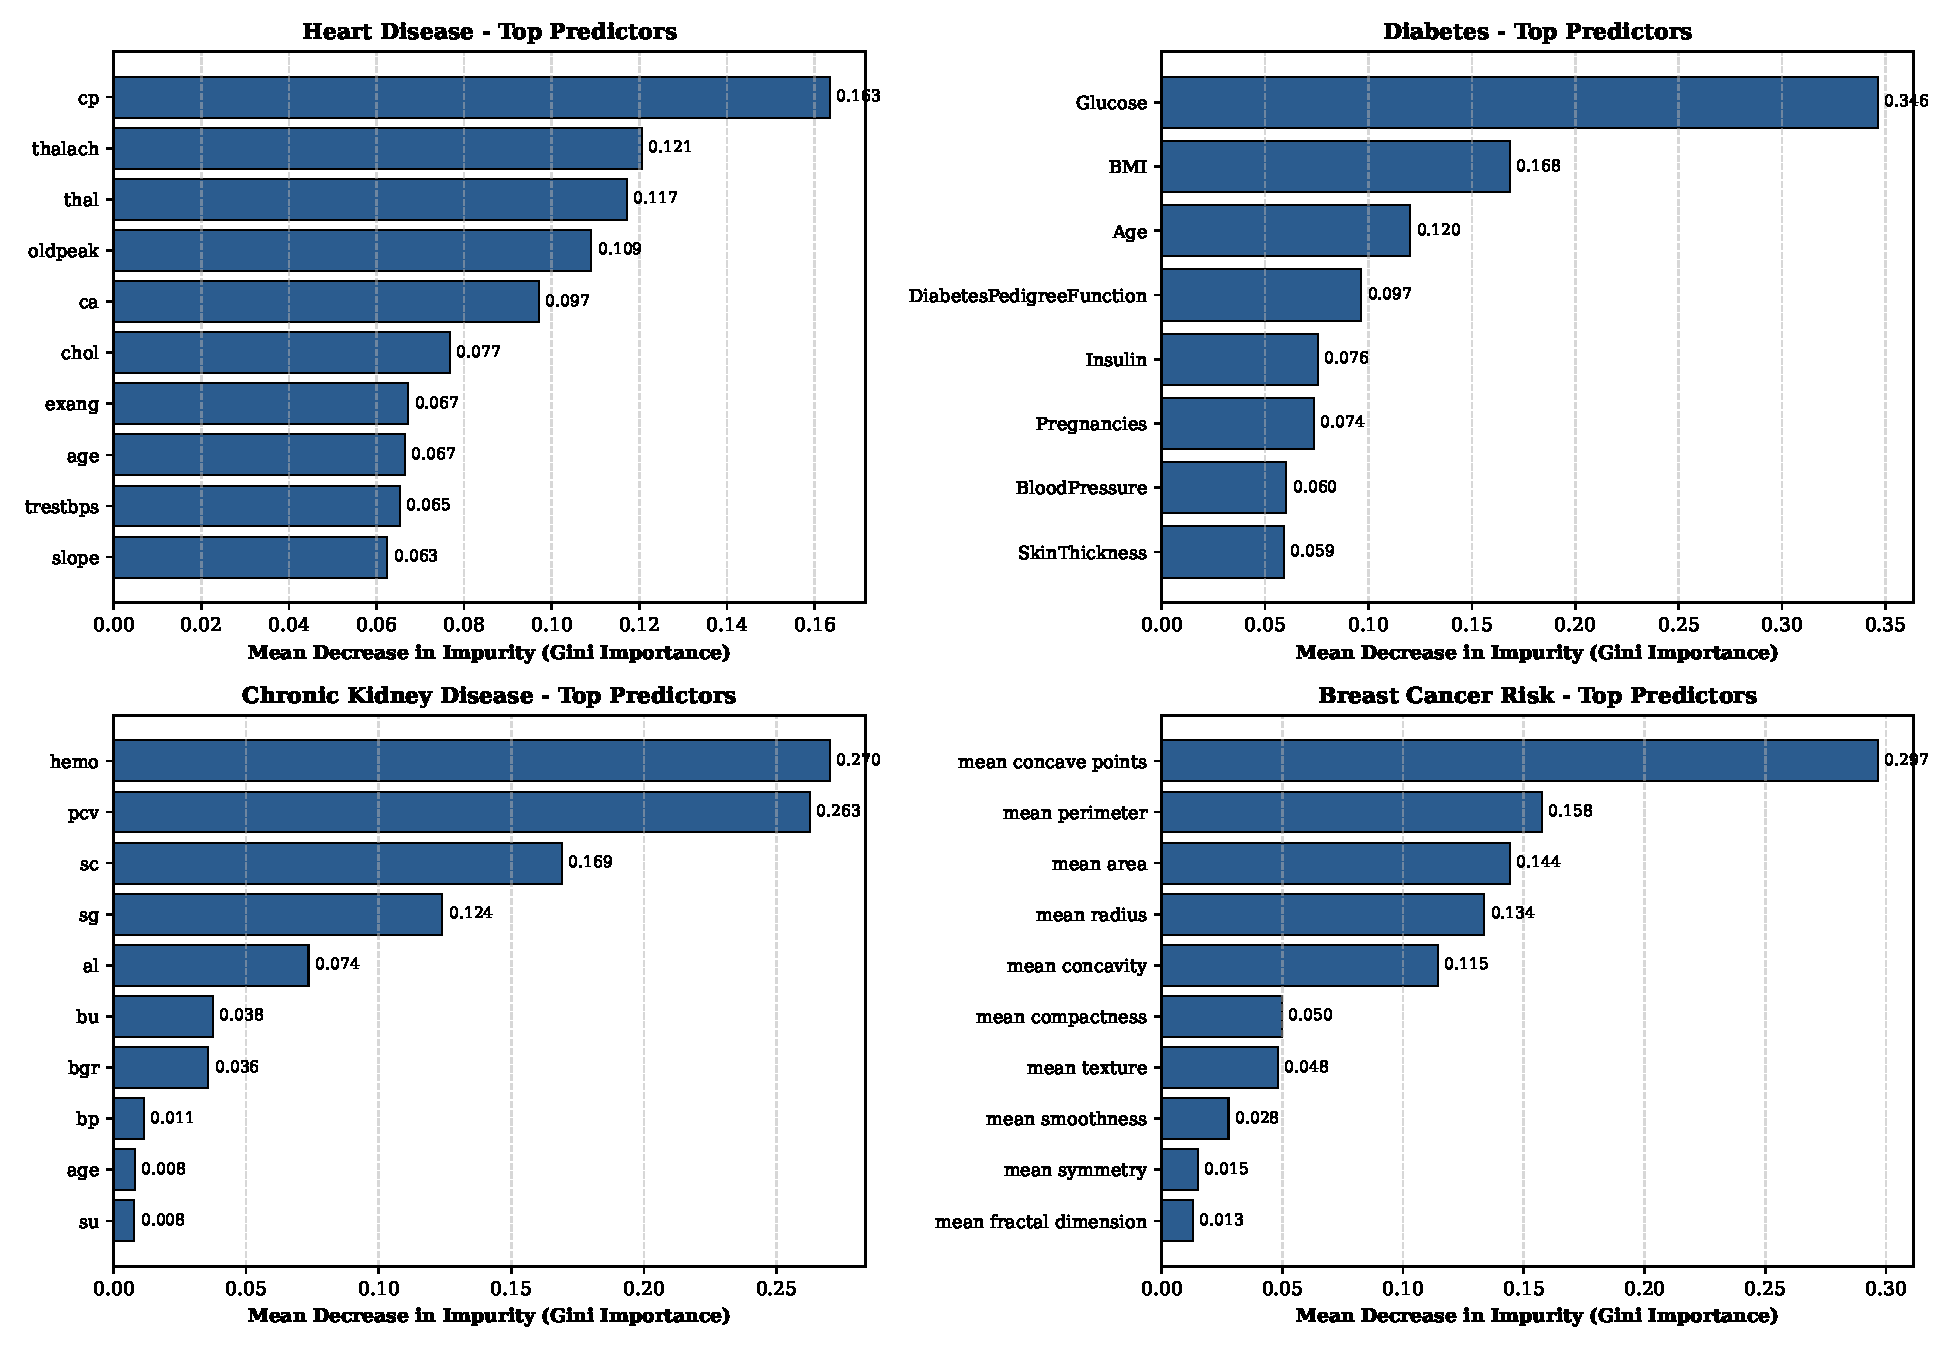
\includegraphics[width=0.92\textwidth]{figures/fig4_feature_importance_analysis.pdf}
    \caption{Mean Decrease in Impurity (Gini Importance) for the top predictive clinical indicators extracted from fitted Random Forest ensembles across four benchmark conditions: (a) Heart Disease (top predictors: maximum heart rate \texttt{thalach}, ST depression \texttt{oldpeak}, chest pain type \texttt{cp}), (b) Chronic Kidney Disease (top predictors: serum creatinine \texttt{sc}, hemoglobin \texttt{hemo}, packed cell volume \texttt{pcv}), (c) Type-2 Diabetes (top predictors: fasting glucose, BMI, age), and (d) Breast Cancer (top predictors: mean concave points, mean perimeter, mean radius). Feature importances are normalized such that $\sum_j J(j) = 1.0$.}
    \label{fig:feature_importance}
\end{figure*}

% Figure 5: Dataset Class Distribution and Imbalance Analysis
\begin{figure*}[htbp]
    \centering
    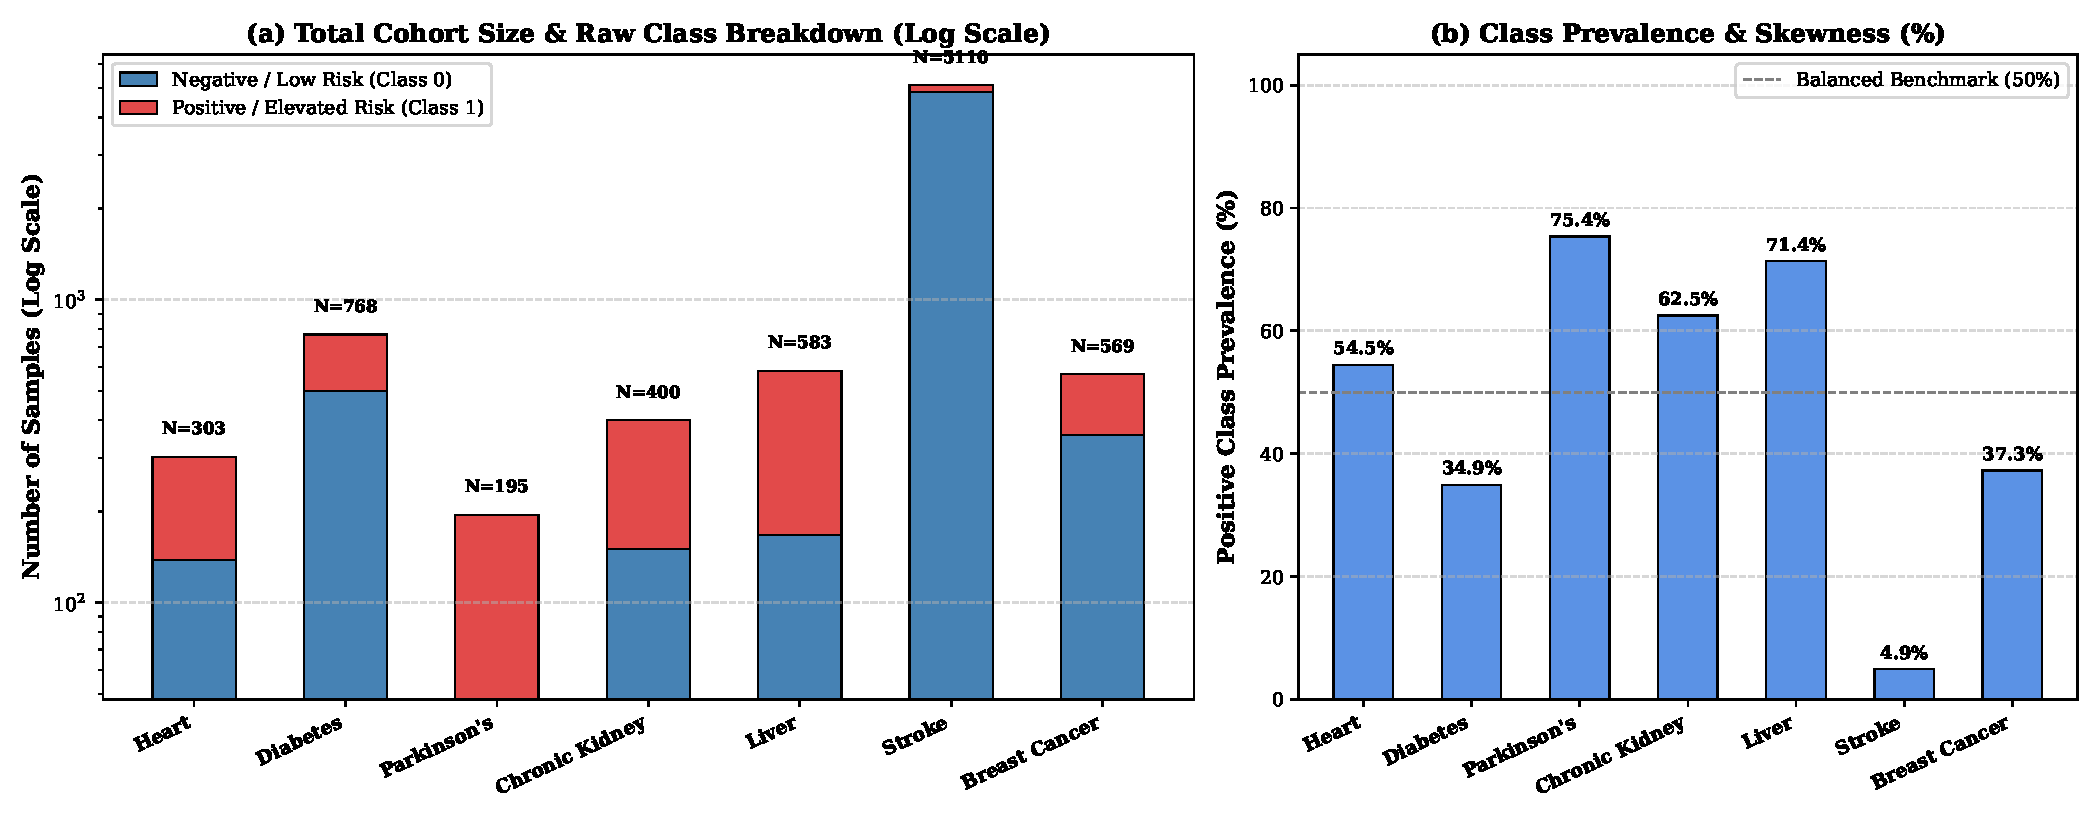
\includegraphics[width=0.95\textwidth]{figures/fig5_class_distribution_and_imbalance.pdf}
    \caption{Dataset scale and class distribution across all seven analyzed clinical cohorts: (a) Total cohort sample sizes ($N$) plotted on a logarithmic scale with negative (healthy/benign) and positive (disease/malignant) stratification, and (b) Observed positive class prevalence (\%) demonstrating significant empirical epidemiological variation, ranging from severe minority imbalance in Stroke Risk ($4.87\%$ prevalence, $N=5,110$) to slight majority prevalence in Chronic Kidney Disease ($62.50\%$) and Parkinson's Disease ($75.38\%$).}
    \label{fig:class_distribution}
\end{figure*}

